\chapter{Les méthodes de travail}

Lorsque un projet devient assez conséquent, sa gestion devient de plus en plus complexe. Un produit informatique comportera un grande quantité de code, dont il faut faciliter la maintenance le plus tôt possible. Il fera intervenir un grand nombre de personnes, réparties dans plusieurs équipes de travail.
En outre, le prestataire devra collaborer avec un client qui n'a pas les mêmes notions techniques et dont les besoins peuvent évoluer.

Une bonne organisation du travail est donc essentielle pour la réussite d'un tel projet.

L'organisation d'un projet passe tout d'abord par une méthode de travail à appliquer. Le choix d'une méthode de travail est généralement la première décision à prendre avec le client avant de commencer le développement d'un produit. En outre, elle aura une grande incidence sur sa réussite.

\section{Mes méthodes de travail dans l'informatique}

Il existe de nombreux modèles de gestion de projet dans le milieu industriel. Nous allons ici nous pencher sur deux méthodes de travail : le cycle en V et les méthodes Agiles.

\subsection{Le cycle en V}

En gestion de projet, il est important de considérer les erreurs comme faisant partie intégrante d'un projet (*Errare Humanum est*). Dans l'industrie en général, plus un problème est détecté tôt, plus il sera facile de le corriger et moins grande en seront les conséquences (effets de bord). Ainsi, pendant le développement d'un produit, l'objectif n'est pas tant de limiter les erreurs, mais davantage de parvenir à les détecter le plus tôt possible.

Le cycle en V est devenu un standard de l'industrie logicielle et dans les autres domaines de l'industrie en général.

Le cycle en V est un modèle de gestion de projet permettant de limiter ces effets de bord, en découpant la réalisation d'un projet en plusieurs étapes de manière séquentielle.

Le cycle en V comporte 3 phases : Conception, Développement et Tests. Chacune de ces phases peut comprendre plusieurs étapes.

On peut noter une correspondances entre les étapes situées sur le même niveau : par exemple, si il existe un problème lors d'un test d'intégration, cela va affecter la conception architecturale. \\

\begin{figure}[h]
   \caption{Schéma du cycle en V}
   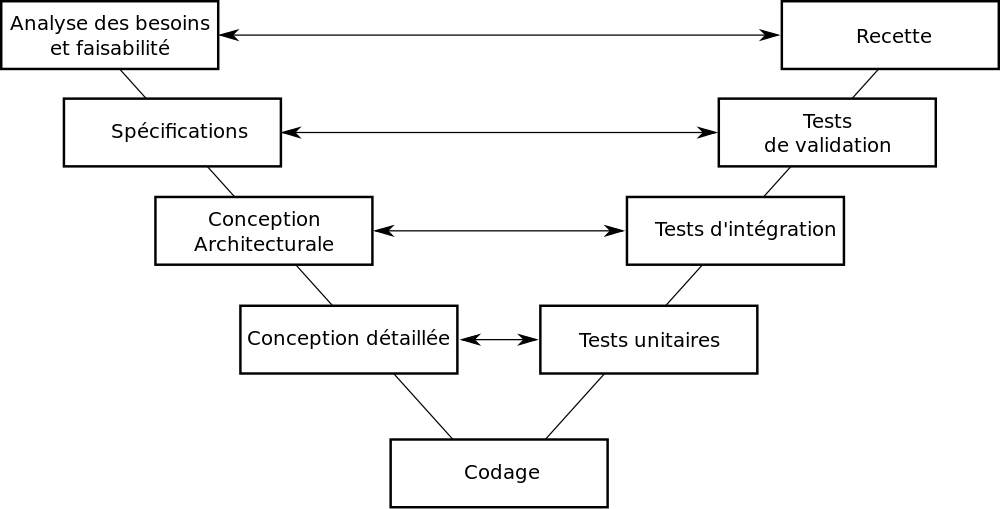
\includegraphics[width=15cm]{img/cycle_en_v.png}
\end{figure}


\begin{itemize}
\item \textbf{La phase de conception}

\begin{itemize}
\item Analyse des besoins et faisabilité ;
\item Spécification ;
\item Conception architecturale ;
\item Conception détaillée.
\end{itemize}

Les étapes de la phases de conception commencent par une approche très globale du projet, et augmentent progressivement le niveau de détail jusqu'à la phase de codage. Chaque étape de conception s'appuie sur l'étape précédente. \\


\item \textbf{La phase de développement logiciel (codage)}
Il s'agit du développement du produit, qui s'appuie sur la conception détaillée. \\

\item \textbf{La phase de tests}

\begin{itemize}
\item Tests unitaires ;
\item Tests d'intégration ;
\item Tests de validation ;
\item Recette.
\end{itemize}

\end{itemize}

Les tests sont des étapes très importantes dans la réalisation d'un produit, car c'est ce qui permet de valider leur bon fonctionnement et la conformité aux attentes du client. Ils commencent par un niveau de détail élevé, puis offrent une vue de plus en plus globale sur le produit final.

Pour la réalisation d'un projet informatique, ce modèle de gestion de projet à l'avantage de prévoir et de quantifier les besoins, de choisir l'architecture logicielle à adopter, de penser à l'intégration des différentes fonctionnalités, avant de commencer son développement. Cela permet notamment d'anticiper certains problèmes de conception pouvant survenir pendant la phase de codage, et donc de réduire développement de fonctionnalités inadaptées.

Par exemple, dans le cadre de la réalisation d'un site Internet, il sera bien utile aux développeurs de savoir que le site devra proposer plusieurs langages avant de commencer la réalisation. En effet, cette fonctionnalité va influencer l'architecture générale du site, et il sera difficile d'implémenter une telle fonctionnalité en cours de développement si elle n'a pas été prévue au départ.

Ainsi, avec une approche théorique, le cycle en V possède de nombreux avantages et peut se révéler très utile dans le développement d'un projet informatique. Toutefois, la mise en pratique de ce modèle de gestion de projet a mis en valeur certains défauts.

\subsection{Les méthodes agiles}

La méthode du cycle en V, bien qu'elle soit intéressante d'un point de vue théorique, possède en réalité de gros inconvénients, pouvant mettre en péril la réussite du projet :

\begin{itemize}

\item Les documents de conception sont réalisés par différentes personnes qui ont chacune leur point de vue. Par ailleurs, il n'y a aucun moyen de vérifier la bonne concordance entre ces différents documents. Ainsi, les développeurs peuvent se trouver face à des incohérences considérables dans le dossier de conception.

\item Les personnes qui réalisent la conception ont souvent un point de vue trop théorique et n'ont pas forcément en tête les problème techniques qui pourront survenir en utilisant leurs choix de conception.

\item La rédaction des différents documents de conception prend du temps et aura donc un impact considérable sur le coût du projet.

\item En cas d'arrêt de la production, pour diverses raison, le produit est inutilisable.

\item Il est courant que le client change d'avis pendant la réalisation 
d'un projet. Avec le modèle du cycle en V, un tel changement impactera toutes les étapes de conception, de développement et de tests, ce qui a une forte incidence sur le coût du projet.

\item Enfin, le problème le plus important du cycle en V est l'effet dit \textbf{Tunnel}. En effet, le client n'a aucune visibilité sur le projet pendant sa réalisation : il est sollicité uniquement au début (pour l'analyse des besoins) et à la fin (pour la recette). Ainsi, si une confusion apparait sur le cahier des charges, le client s'en apercevra uniquement pendant la recette. En prenant également en compte les confusions pouvant exister entre les différentes étapes de conception, le client peut se retrouver face à un produit ne correspondant pas du tout à ses attentes.\\

\end{itemize}

Ainsi, l'industrie informatique a parfois connu des scénarios catastrophiques en utilisant la méthode du cycle en V. Dès lors, pour limiter ces dangers, d'autres modèles de gestion de projet ont vu le jour.

Les méthodes agiles, apparues dans les années 1990, sont un groupe de pratiques de développement de projets informatiques reposant sur un même philosophie.

Elles consistent à développer le produit de manière \textbf{itérative, incrémentale et adaptative}. Les fonctionnalités sont développées les unes après les autres, les plus importantes en premier. Le client est sollicité régulièrement afin de vérifier la conformité entre ses attentes avec ce qui a été développé.

En outre, les méthodes agiles permettent :

\begin{itemize}
\item une bonne conformité entre les attentes du client et le produit développé ;
\item une grande réactivité à ses demandes, même pendant la réalisation du produit ;
\item d'obtenir un produit partiellement fonctionnel, quelque soit l'état d'avancement du projet.
\end{itemize}

\begin{figure}[h]
   \caption{Schéma du circuit agile}
   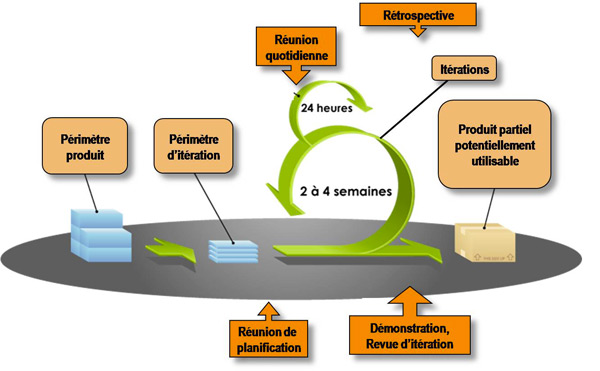
\includegraphics[width=15cm]{img/agiles.jpg}
\end{figure}

Il existe plusieurs méthodes Agiles, qui ont leurs propres spécifications et qui doivent être adaptées en fonction du contexte. Ainsi, il ne suffit pas de choisir de développer un projet au moyen des méthodes agiles, il faut également se pencher sur la méthode à adopter. Parmi les plus connues, on retrouve :

\subsubsection{La méthode Scrum}

Le terme *Scrum* (signifiant « mêlée ») provient du rugby à XV, sport qui a pour objectif d'atteindre un but grace à une équipe soudée.
Le projet est découpé en plusieurs phases appelées *sprints*, pendant lesquelles l'équipe a comme objectif de développer un ensemble précis de fonctionnalités. À la fin de chaque sprint, l'équipe se retrouve pour une réunion appelée *revue de sprint*, pendant laquelle les membres valident ensemble les fonctionnalités développées et préparent celles du prochain sprint.

Les fonctionnalités sont souvent représentées physiquement au moyen de *Post-its* à coller sur un tableau composé de trois colonnes correspondant à leur état d'avancement : *à faire*, *en cours* et *réalisé*. Au sein de l'équipe, une personne désignée *ScrumMaster* a la charge de motiver l'équipe, de vérifier les tâches développées et proposer celles du prochain sprint, ainsi que de former le directeur de produit et l'équipe à la méthode Scrum. Ce statut n'a aucune signification hierarchique et un nouveau ScrumMaster peut être désigné à chaque sprint.

Cette méthode facilite le dynamisme et le travail d'équipe, elle est adaptée aux projets qui peuvent évoluer.
{en quoi cette méthode répond t elle au besoin d'evolutivité des projets ?}

\subsubsection{La méthode XP (Extreme programming)}

La méthode XP consiste en différents principes à appliquer pendant la réalisation d'un projet. Ces derniers existent depuis de nombreuses années, toutefois ils sont ici poussés à l'extrême :

Extrait de \textit{Extreme Programming Explained} :
\begin{italicquotes}
\begin{itemize}
\item Puisque la revue de code est une bonne pratique, elle sera faite en permanence (par un binôme) ;
\item puisque les tests sont utiles, ils seront faits systématiquement avant chaque mise en œuvre ;
\item puisque la conception est importante, elle sera faite tout au long du projet (refactoring) ;
\item puisque la simplicité permet d'avancer plus vite, nous choisirons toujours la solution la plus simple ;
\item puisque la compréhension est importante, nous définirons et ferons évoluer ensemble des métaphores ;
\item puisque l'intégration des modifications est cruciale, nous l'effectuerons plusieurs fois par jour ;
\item puisque les besoins évoluent vite, nous ferons des cycles de développement très rapides pour nous adapter au changement.
\end{itemize}
\end{italicquotes}
Cette méthode est adaptée aux équipes réduites avec des besoins qui peuvent évoluer.

\section{Critères de choix}

\subsection{Rapport avec le client}
\subsection{Préférences au sein de l'entreprise}

\section{Conclusion}

Nous avons vu les différentes méthodes de travail pouvant être adoptées pour la réalisation d'un projet informatique. Nous avons également vu comment le rapport avec le client et les préférences au sein de l'entreprise peuvent influencer le choix de ces méthodes.